% sections/04_background_tagging.tex: generated by newdeck/html2beamer.py from the HTML deck, then edited by hand

% ---------------------------------------------------------------- slide 19: Outline
\begin{btframe}{}{Outline}
\begin{outlinelist}
\outlineitem{1}{Introduction}{the background types, the geometry, the input muons and neutrinos}{0.35}
\outlineitem{2}{Simulation}{transport, inelastic scattering, technologies, hits and digitisation, signal generation}{0.35}
\outlineitem{3}{Selection}{track cuts, pair cuts and time coincidence}{0.35}
\outlineitem{4}{Backgrounds before tagging}{μ and ν inelastic scattering, MS7 K\textsubscript{L}, combinatorial pairs}{0.35}
\outlineitem{5}{Background tagging}{rules, V0 rule, SBT model, R1–R3, Z2–Z3, summary}{1.00}
\outlineitem{6}{Optimisation and conclusion}{genetic-algorithm search, the optimised design}{0.35}
\end{outlinelist}
\end{btframe}

% ---------------------------------------------------------------- slide 20: The reference designs R1, R2, R3
\begin{btframe}{5 · Background tagging · designs}{The reference designs R1, R2, R3}
\noindent \begin{minipage}[c]{40.97pt}\raggedright
{\fontsize{6.37pt}{8.60pt}\selectfont \textcolor{cern}{\textbf{R1}}\par}
\vspace{2.46pt}
{\fontsize{5.01pt}{6.76pt}\selectfont 99.7 drachmas\par}
\end{minipage}%
\hfill%
\begin{minipage}[c]{\dimexpr(1.0000\linewidth-1.0000\dimexpr46.09pt\relax)}\raggedright
{\centering {\renewcommand{\skubtlabel}{UBT: straws 1 × 2.7 m\textsuperscript{2} (4.8 dr) + tiles 4 × 4 m\textsuperscript{2}, 2 × 2 cm\textsuperscript{2} flames (94.8 dr)}\designsketch[52.35pt]{}{0}{}}\par}
\end{minipage}\par
\vspace{2.46pt}
\noindent \begin{minipage}[c]{40.97pt}\raggedright
{\fontsize{6.37pt}{8.60pt}\selectfont \textcolor{cern}{\textbf{R2}}\par}
\vspace{2.46pt}
{\fontsize{5.01pt}{6.76pt}\selectfont 333.5 drachmas = budget\newline{}\textcolor{purple}{+ V0 rule}\par}
\end{minipage}%
\hfill%
\begin{minipage}[c]{\dimexpr(1.0000\linewidth-1.0000\dimexpr46.09pt\relax)}\raggedright
{\centering {\renewcommand{\skubtlabel}{UBT: straws 1 × 2.7 m\textsuperscript{2} (4.8 dr) + tiles 4 × 4 m\textsuperscript{2}, 2 × 2 cm\textsuperscript{2} flames (94.8 dr)}\designsketch[52.35pt]{0,...,9}{0}{SBT: 854 LS cells, 20 cm, 10 rings (233.8 dr)}}\par}
\end{minipage}\par
\vspace{2.46pt}
\noindent \begin{minipage}[c]{40.97pt}\raggedright
{\fontsize{6.37pt}{8.60pt}\selectfont \textcolor{cern}{\textbf{R3}}\par}
\vspace{2.46pt}
{\fontsize{5.01pt}{6.76pt}\selectfont 378.7 drachmas\newline{}\textcolor{purple}{+ V0 rule}\par}
\end{minipage}%
\hfill%
\begin{minipage}[c]{\dimexpr(1.0000\linewidth-1.0000\dimexpr46.09pt\relax)}\raggedright
{\centering {\renewcommand{\skubtlabel}{UBT: straws 1 × 2.7 m\textsuperscript{2} (4.8 dr) + tiles 4 × 4 m\textsuperscript{2}, 2 × 2 cm\textsuperscript{2} flames (94.8 dr)}\renewcommand{\skmsmslabel}{MSMS: 24 Si stations\\30 × 30 cm\textsuperscript{2} (45.2 dr)}\designsketch[52.35pt]{0,...,9}{1}{SBT: 854 LS cells, 20 cm, 10 rings (233.8 dr)}}\par}
\end{minipage}\par
\end{btframe}

% ---------------------------------------------------------------- slide 21: How a candidate is tagged: tracks, neutrals, MS7
\begin{btframe}{5 · Background tagging · tagging chain}{How a candidate is tagged: tracks, neutrals, MS7}
{\fontsize{5.23pt}{7.07pt}\selectfont \textbf{Tracks: does a measured track come from upstream?}\par}
\vspace{2.46pt}
\begin{flowrow}{\dimexpr(\linewidth-3\dimexpr6.37pt\relax)/4\relax}{6.37pt}%
\flowstep{white}{rule}{2.28pt}{3.64pt}{{\fontsize{5.92pt}{7.40pt}\selectfont\textbf{\textcolor{cern}{candidate}}\par}\vspace{0.91pt}{\fontsize{5.01pt}{6.76pt}\selectfont\textcolor{ink}{2 tracks, vertex in the vessel}\par}}%
\flowarrow%
\flowstep{white}{rule}{2.28pt}{3.64pt}{{\fontsize{5.92pt}{7.40pt}\selectfont\textbf{\textcolor{cern}{each track back}}\par}\vspace{0.91pt}{\fontsize{5.01pt}{6.76pt}\selectfont\textcolor{ink}{straight line from SST1 to every plane upstream of the vertex}\par}}%
\flowarrow%
\flowstep{white}{rule}{2.28pt}{3.64pt}{{\fontsize{5.92pt}{7.40pt}\selectfont\textbf{\textcolor{cern}{window}}\par}\vspace{0.91pt}{\fontsize{5.01pt}{6.76pt}\selectfont\textcolor{ink}{r = 5 cm + (0.5 mrad + 6 mrad·GeV/p)·Δz, ±3σ in time; SBT along the wall}\par}}%
\flowarrow%
\flowstep{white}{rule}{2.28pt}{3.64pt}{{\fontsize{5.92pt}{7.40pt}\selectfont\textbf{\textcolor{cern}{hit?}}\par}\vspace{0.91pt}{\fontsize{5.01pt}{6.76pt}\selectfont\textcolor{ink}{yes → tagged (+ bounce search from the cavern wall)}\par}}%
\end{flowrow}
\vspace{2.46pt}
{\fontsize{5.23pt}{7.07pt}\selectfont \textcolor{purple}{\textbf{Neutrals (V0 rule, R2 and R3): was the candidate made upstream?}}\par}
\vspace{2.46pt}
\begin{flowrow}{\dimexpr(\linewidth-3\dimexpr6.37pt\relax)/4\relax}{6.37pt}%
\flowstep{white}{rule}{2.28pt}{3.64pt}{{\fontsize{5.92pt}{7.40pt}\selectfont\textbf{\textcolor{purple}{candidate}}\par}\vspace{0.91pt}{\fontsize{5.01pt}{6.76pt}\selectfont\textcolor{ink}{p\textsubscript{vis} = p\textsubscript{1} + p\textsubscript{2} < 20 GeV}\par}}%
\flowarrow%
\flowstep{white}{rule}{2.28pt}{3.64pt}{{\fontsize{5.92pt}{7.40pt}\selectfont\textbf{\textcolor{purple}{trace back as a neutral}}\par}\vspace{0.91pt}{\fontsize{5.01pt}{6.76pt}\selectfont\textcolor{ink}{from the vertex along p\textsubscript{vis} to the UBT}\par}}%
\flowarrow%
\flowstep{white}{rule}{2.28pt}{3.64pt}{{\fontsize{5.92pt}{7.40pt}\selectfont\textbf{\textcolor{purple}{disc + early window}}\par}\vspace{0.91pt}{\fontsize{5.01pt}{6.76pt}\selectfont\textcolor{ink}{r = 5 cm + max(25 mrad, 0.25 GeV/p\textsubscript{vis})·Δz; window opened by the K\textsubscript{L} flight time}\par}}%
\flowarrow%
\flowstep{white}{rule}{2.28pt}{3.64pt}{{\fontsize{5.92pt}{7.40pt}\selectfont\textbf{\textcolor{purple}{any hit?}}\par}\vspace{0.91pt}{\fontsize{5.01pt}{6.76pt}\selectfont\textcolor{ink}{yes → tagged: the parent muon or the other products}\par}}%
\end{flowrow}
\vspace{2.46pt}
{\fontsize{5.23pt}{7.07pt}\selectfont \textcolor{red}{\textbf{MS7 (MSMS, R3): did the interaction happen in the last iron?}}\par}
\vspace{2.46pt}
\begin{flowrow}{\dimexpr(\linewidth-3\dimexpr6.37pt\relax)/4\relax}{6.37pt}%
\flowstep{white}{rule}{2.28pt}{3.64pt}{{\fontsize{5.92pt}{7.40pt}\selectfont\textbf{\textcolor{red}{candidate}}\par}\vspace{0.91pt}{\fontsize{5.01pt}{6.76pt}\selectfont\textcolor{ink}{traced back as a neutral}\par}}%
\flowarrow%
\flowstep{white}{rule}{2.28pt}{3.64pt}{{\fontsize{5.92pt}{7.40pt}\selectfont\textbf{\textcolor{red}{strip layers}}\par}\vspace{0.91pt}{\fontsize{5.01pt}{6.76pt}\selectfont\textcolor{ink}{29.39 / 29.59 / 29.79 m, 24 stations}\par}}%
\flowarrow%
\flowstep{white}{rule}{2.28pt}{3.64pt}{{\fontsize{5.92pt}{7.40pt}\selectfont\textbf{\textcolor{red}{disc}}\par}\vspace{0.91pt}{\fontsize{5.01pt}{6.76pt}\selectfont\textcolor{ink}{2 cm + 10 mrad·Δz, ±1.5 ns}\par}}%
\flowarrow%
\flowstep{white}{rule}{2.28pt}{3.64pt}{{\fontsize{5.92pt}{7.40pt}\selectfont\textbf{\textcolor{red}{own products?}}\par}\vspace{0.91pt}{\fontsize{5.01pt}{6.76pt}\selectfont\textcolor{ink}{yes → tagged}\par}}%
\end{flowrow}
\slidenote{Source: veto lib/veto/reco.py v0\_tag (16–17 Nov 2026); numbers results\_rerun/reco/r123\_study\_v0statk\_1622cf7.json (bin/v0rule\_study.py, V0-enriched MS7 samples, full selection).}
\end{btframe}

% ---------------------------------------------------------------- slide 22: How a candidate is tagged: tracks
\begin{btframe}{5 · Background tagging · tagging chain 1/3}{How a candidate is tagged: tracks}
\noindent \begin{minipage}[c]{38.69pt}\raggedright
{\fontsize{4.32pt}{5.84pt}\selectfont \textcolor{cern}{\textbf{Tracks}}\par}
\end{minipage}%
\hfill%
\begin{minipage}[c]{\dimexpr(1.0000\linewidth-1.0000\dimexpr42.90pt\relax)}\raggedright
\begin{flowrow}{\dimexpr(\linewidth-3\dimexpr5.46pt\relax)/4\relax}{5.46pt}%
\flowstep{cern}{cern}{2.28pt}{3.64pt}{{\fontsize{4.78pt}{5.97pt}\selectfont\textbf{\textcolor{white}{candidate}}\par}\vspace{0.91pt}{\fontsize{4.10pt}{5.53pt}\selectfont\textcolor{white}{2 tracks, vertex in the vessel}\par}}%
\flowarrow%
\flowstep{cern}{cern}{2.28pt}{3.64pt}{{\fontsize{4.78pt}{5.97pt}\selectfont\textbf{\textcolor{white}{each track back}}\par}\vspace{0.91pt}{\fontsize{4.10pt}{5.53pt}\selectfont\textcolor{white}{straight line from SST1 upstream}\par}}%
\flowarrow%
\flowstep{cern}{cern}{2.28pt}{3.64pt}{{\fontsize{4.78pt}{5.97pt}\selectfont\textbf{\textcolor{white}{window}}\par}\vspace{0.91pt}{\fontsize{4.10pt}{5.53pt}\selectfont\textcolor{white}{r = 5 cm + (0.5 + 6 GeV/p) mrad·Δz, ±3σ}\par}}%
\flowarrow%
\flowstep{cern}{cern}{2.28pt}{3.64pt}{{\fontsize{4.78pt}{5.97pt}\selectfont\textbf{\textcolor{white}{hit?}}\par}\vspace{0.91pt}{\fontsize{4.10pt}{5.53pt}\selectfont\textcolor{white}{yes → tagged}\par}}%
\end{flowrow}
\end{minipage}\par
\vspace{2.46pt}
\fadeblock{0.28}{\noindent \begin{minipage}[c]{38.69pt}\raggedright
{\fontsize{4.32pt}{5.84pt}\selectfont \textcolor{purple}{\textbf{Neutrals (V0 rule, R2, R3)}}\par}
\end{minipage}%
\hfill%
\begin{minipage}[c]{\dimexpr(1.0000\linewidth-1.0000\dimexpr42.90pt\relax)}\raggedright
\begin{flowrow}{\dimexpr(\linewidth-3\dimexpr5.46pt\relax)/4\relax}{5.46pt}%
\flowstep{white}{rule}{2.28pt}{3.64pt}{{\fontsize{4.78pt}{5.97pt}\selectfont\textbf{\textcolor{purple}{candidate}}\par}\vspace{0.91pt}{\fontsize{4.10pt}{5.53pt}\selectfont\textcolor{ink}{p\textsubscript{vis} < 20 GeV}\par}}%
\flowarrow%
\flowstep{white}{rule}{2.28pt}{3.64pt}{{\fontsize{4.78pt}{5.97pt}\selectfont\textbf{\textcolor{purple}{trace back as a neutral}}\par}\vspace{0.91pt}{\fontsize{4.10pt}{5.53pt}\selectfont\textcolor{ink}{vertex → UBT along p\textsubscript{vis}}\par}}%
\flowarrow%
\flowstep{white}{rule}{2.28pt}{3.64pt}{{\fontsize{4.78pt}{5.97pt}\selectfont\textbf{\textcolor{purple}{disc + early window}}\par}\vspace{0.91pt}{\fontsize{4.10pt}{5.53pt}\selectfont\textcolor{ink}{5 cm + max(25, 250/p\textsubscript{vis}) mrad·Δz}\par}}%
\flowarrow%
\flowstep{white}{rule}{2.28pt}{3.64pt}{{\fontsize{4.78pt}{5.97pt}\selectfont\textbf{\textcolor{purple}{any hit?}}\par}\vspace{0.91pt}{\fontsize{4.10pt}{5.53pt}\selectfont\textcolor{ink}{yes → tagged}\par}}%
\end{flowrow}
\end{minipage}\par
}\vspace{2.46pt}
\fadeblock{0.28}{\noindent \begin{minipage}[c]{38.69pt}\raggedright
{\fontsize{4.32pt}{5.84pt}\selectfont \textcolor{red}{\textbf{MS7 (MSMS, R3)}}\par}
\end{minipage}%
\hfill%
\begin{minipage}[c]{\dimexpr(1.0000\linewidth-1.0000\dimexpr42.90pt\relax)}\raggedright
\begin{flowrow}{\dimexpr(\linewidth-3\dimexpr5.46pt\relax)/4\relax}{5.46pt}%
\flowstep{white}{rule}{2.28pt}{3.64pt}{{\fontsize{4.78pt}{5.97pt}\selectfont\textbf{\textcolor{red}{candidate}}\par}\vspace{0.91pt}{\fontsize{4.10pt}{5.53pt}\selectfont\textcolor{ink}{traced back as a neutral}\par}}%
\flowarrow%
\flowstep{white}{rule}{2.28pt}{3.64pt}{{\fontsize{4.78pt}{5.97pt}\selectfont\textbf{\textcolor{red}{strip layers}}\par}\vspace{0.91pt}{\fontsize{4.10pt}{5.53pt}\selectfont\textcolor{ink}{29.39 / 29.59 / 29.79 m}\par}}%
\flowarrow%
\flowstep{white}{rule}{2.28pt}{3.64pt}{{\fontsize{4.78pt}{5.97pt}\selectfont\textbf{\textcolor{red}{disc}}\par}\vspace{0.91pt}{\fontsize{4.10pt}{5.53pt}\selectfont\textcolor{ink}{2 cm + 10 mrad·Δz, ±1.5 ns}\par}}%
\flowarrow%
\flowstep{white}{rule}{2.28pt}{3.64pt}{{\fontsize{4.78pt}{5.97pt}\selectfont\textbf{\textcolor{red}{own products?}}\par}\vspace{0.91pt}{\fontsize{4.10pt}{5.53pt}\selectfont\textcolor{ink}{yes → tagged}\par}}%
\end{flowrow}
\end{minipage}\par
}\vspace{2.46pt}
\noindent \begin{minipage}[c]{\dimexpr(0.6000\linewidth-0.6000\dimexpr7.85pt\relax)}\raggedright
{\centering 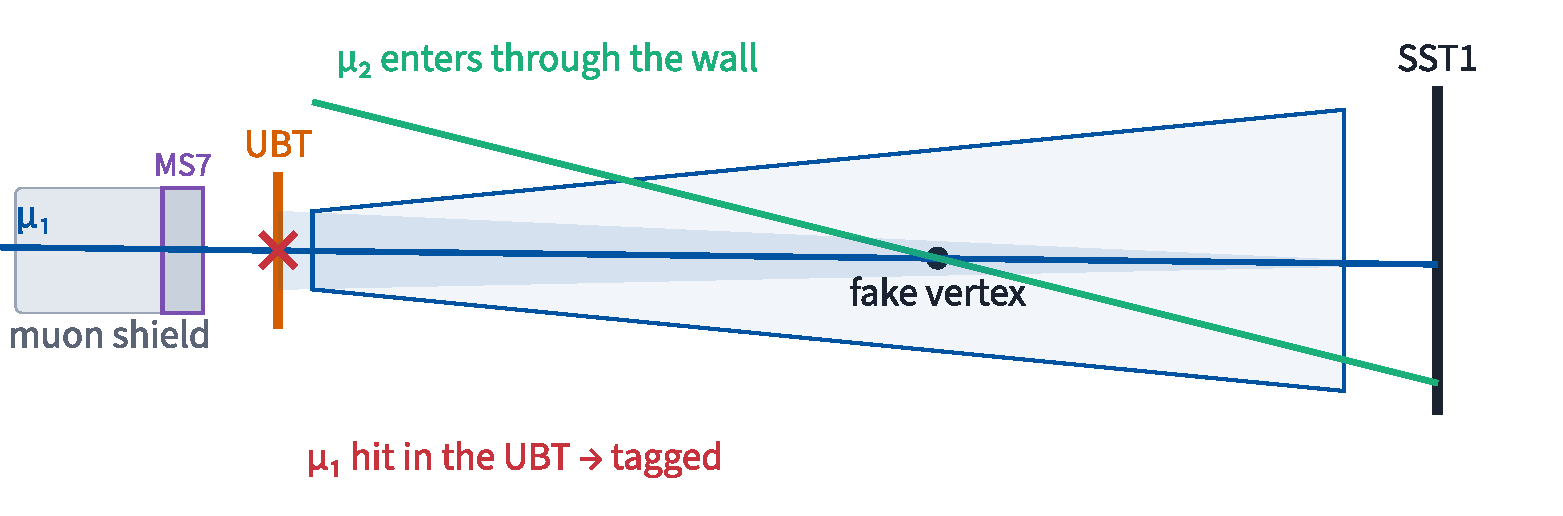
\includegraphics[width=1.00\linewidth,height=45.52pt,keepaspectratio]{figs/s21_sk1.pdf}\par}
\end{minipage}%
\hfill%
\begin{minipage}[c]{\dimexpr(0.4000\linewidth-0.4000\dimexpr7.85pt\relax)}\raggedright
\begin{mathbox}[cern]{5.23pt}
\textbf{window at each plane}\newline{}r = 5 cm + (0.5 mrad + 6 mrad·GeV / p) · Δz\newline{}|t\textsubscript{hit} − t\textsubscript{track}| < 3σ\textsubscript{t}\newline{}\textcolor{muted}{Δz: from SST1 back to the plane}\newline{}p = 10 GeV: r ≈ \textbf{11 cm}; p = 1 GeV: r ≈ \textbf{38 cm} at the UBT
\end{mathbox}
\end{minipage}\par
\vspace{2.46pt}
\noindent \begin{minipage}[c]{\dimexpr(0.6154\linewidth-0.6154\dimexpr7.85pt\relax)}\raggedright
{\centering 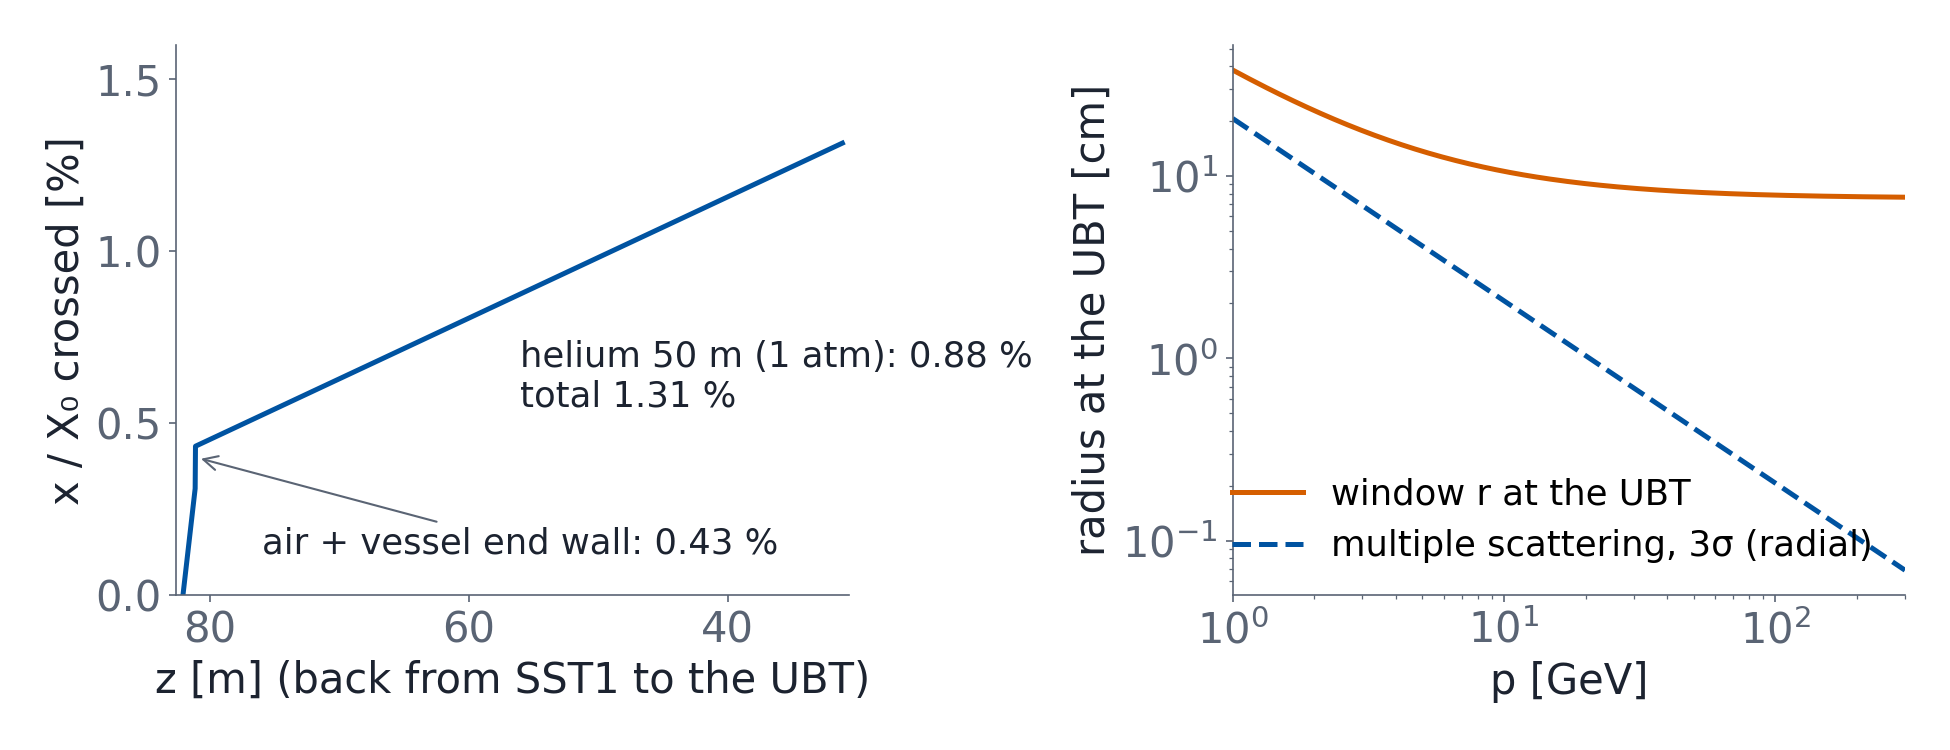
\includegraphics[height=72.83pt,keepaspectratio]{figs/s21_img2.png}\par}
\end{minipage}%
\hfill%
\begin{minipage}[c]{\dimexpr(0.3846\linewidth-0.3846\dimexpr7.85pt\relax)}\raggedright
{\fontsize{4.55pt}{6.15pt}\selectfont Back from SST1 to the UBT a track crosses \textbf{1.3 \% X\textsubscript{0}} (air, vessel end wall, 50 m of helium). Its multiple scattering (Highland, 3σ) stays inside the window at every momentum: \textbf{21 cm vs 38 cm} at 1 GeV. A hit in the window and ±3σ in time → \textbf{tagged}.\par}
\end{minipage}\par
\end{btframe}

% ---------------------------------------------------------------- slide 23: How a candidate is tagged: neutrals (V0 rule)
\begin{btframe}{5 · Background tagging · tagging chain 2/3}{How a candidate is tagged: neutrals (V0 rule)}
\fadeblock{0.28}{\noindent \begin{minipage}[c]{38.69pt}\raggedright
{\fontsize{4.32pt}{5.84pt}\selectfont \textcolor{cern}{\textbf{Tracks}}\par}
\end{minipage}%
\hfill%
\begin{minipage}[c]{\dimexpr(1.0000\linewidth-1.0000\dimexpr42.90pt\relax)}\raggedright
\begin{flowrow}{\dimexpr(\linewidth-3\dimexpr5.46pt\relax)/4\relax}{5.46pt}%
\flowstep{white}{rule}{2.28pt}{3.64pt}{{\fontsize{4.78pt}{5.97pt}\selectfont\textbf{\textcolor{cern}{candidate}}\par}\vspace{0.91pt}{\fontsize{4.10pt}{5.53pt}\selectfont\textcolor{ink}{2 tracks, vertex in the vessel}\par}}%
\flowarrow%
\flowstep{white}{rule}{2.28pt}{3.64pt}{{\fontsize{4.78pt}{5.97pt}\selectfont\textbf{\textcolor{cern}{each track back}}\par}\vspace{0.91pt}{\fontsize{4.10pt}{5.53pt}\selectfont\textcolor{ink}{straight line from SST1 upstream}\par}}%
\flowarrow%
\flowstep{white}{rule}{2.28pt}{3.64pt}{{\fontsize{4.78pt}{5.97pt}\selectfont\textbf{\textcolor{cern}{window}}\par}\vspace{0.91pt}{\fontsize{4.10pt}{5.53pt}\selectfont\textcolor{ink}{r = 5 cm + (0.5 + 6 GeV/p) mrad·Δz, ±3σ}\par}}%
\flowarrow%
\flowstep{white}{rule}{2.28pt}{3.64pt}{{\fontsize{4.78pt}{5.97pt}\selectfont\textbf{\textcolor{cern}{hit?}}\par}\vspace{0.91pt}{\fontsize{4.10pt}{5.53pt}\selectfont\textcolor{ink}{yes → tagged}\par}}%
\end{flowrow}
\end{minipage}\par
}\vspace{2.46pt}
\noindent \begin{minipage}[c]{38.69pt}\raggedright
{\fontsize{4.32pt}{5.84pt}\selectfont \textcolor{purple}{\textbf{Neutrals (V0 rule, R2, R3)}}\par}
\end{minipage}%
\hfill%
\begin{minipage}[c]{\dimexpr(1.0000\linewidth-1.0000\dimexpr42.90pt\relax)}\raggedright
\begin{flowrow}{\dimexpr(\linewidth-3\dimexpr5.46pt\relax)/4\relax}{5.46pt}%
\flowstep{purple}{purple}{2.28pt}{3.64pt}{{\fontsize{4.78pt}{5.97pt}\selectfont\textbf{\textcolor{white}{candidate}}\par}\vspace{0.91pt}{\fontsize{4.10pt}{5.53pt}\selectfont\textcolor{white}{p\textsubscript{vis} < 20 GeV}\par}}%
\flowarrow%
\flowstep{purple}{purple}{2.28pt}{3.64pt}{{\fontsize{4.78pt}{5.97pt}\selectfont\textbf{\textcolor{white}{trace back as a neutral}}\par}\vspace{0.91pt}{\fontsize{4.10pt}{5.53pt}\selectfont\textcolor{white}{vertex → UBT along p\textsubscript{vis}}\par}}%
\flowarrow%
\flowstep{purple}{purple}{2.28pt}{3.64pt}{{\fontsize{4.78pt}{5.97pt}\selectfont\textbf{\textcolor{white}{disc + early window}}\par}\vspace{0.91pt}{\fontsize{4.10pt}{5.53pt}\selectfont\textcolor{white}{5 cm + max(25, 250/p\textsubscript{vis}) mrad·Δz}\par}}%
\flowarrow%
\flowstep{purple}{purple}{2.28pt}{3.64pt}{{\fontsize{4.78pt}{5.97pt}\selectfont\textbf{\textcolor{white}{any hit?}}\par}\vspace{0.91pt}{\fontsize{4.10pt}{5.53pt}\selectfont\textcolor{white}{yes → tagged}\par}}%
\end{flowrow}
\end{minipage}\par
\vspace{2.46pt}
\fadeblock{0.28}{\noindent \begin{minipage}[c]{38.69pt}\raggedright
{\fontsize{4.32pt}{5.84pt}\selectfont \textcolor{red}{\textbf{MS7 (MSMS, R3)}}\par}
\end{minipage}%
\hfill%
\begin{minipage}[c]{\dimexpr(1.0000\linewidth-1.0000\dimexpr42.90pt\relax)}\raggedright
\begin{flowrow}{\dimexpr(\linewidth-3\dimexpr5.46pt\relax)/4\relax}{5.46pt}%
\flowstep{white}{rule}{2.28pt}{3.64pt}{{\fontsize{4.78pt}{5.97pt}\selectfont\textbf{\textcolor{red}{candidate}}\par}\vspace{0.91pt}{\fontsize{4.10pt}{5.53pt}\selectfont\textcolor{ink}{traced back as a neutral}\par}}%
\flowarrow%
\flowstep{white}{rule}{2.28pt}{3.64pt}{{\fontsize{4.78pt}{5.97pt}\selectfont\textbf{\textcolor{red}{strip layers}}\par}\vspace{0.91pt}{\fontsize{4.10pt}{5.53pt}\selectfont\textcolor{ink}{29.39 / 29.59 / 29.79 m}\par}}%
\flowarrow%
\flowstep{white}{rule}{2.28pt}{3.64pt}{{\fontsize{4.78pt}{5.97pt}\selectfont\textbf{\textcolor{red}{disc}}\par}\vspace{0.91pt}{\fontsize{4.10pt}{5.53pt}\selectfont\textcolor{ink}{2 cm + 10 mrad·Δz, ±1.5 ns}\par}}%
\flowarrow%
\flowstep{white}{rule}{2.28pt}{3.64pt}{{\fontsize{4.78pt}{5.97pt}\selectfont\textbf{\textcolor{red}{own products?}}\par}\vspace{0.91pt}{\fontsize{4.10pt}{5.53pt}\selectfont\textcolor{ink}{yes → tagged}\par}}%
\end{flowrow}
\end{minipage}\par
}\vspace{2.46pt}
\noindent \begin{minipage}[c]{\dimexpr(0.6000\linewidth-0.6000\dimexpr7.85pt\relax)}\raggedright
{\centering 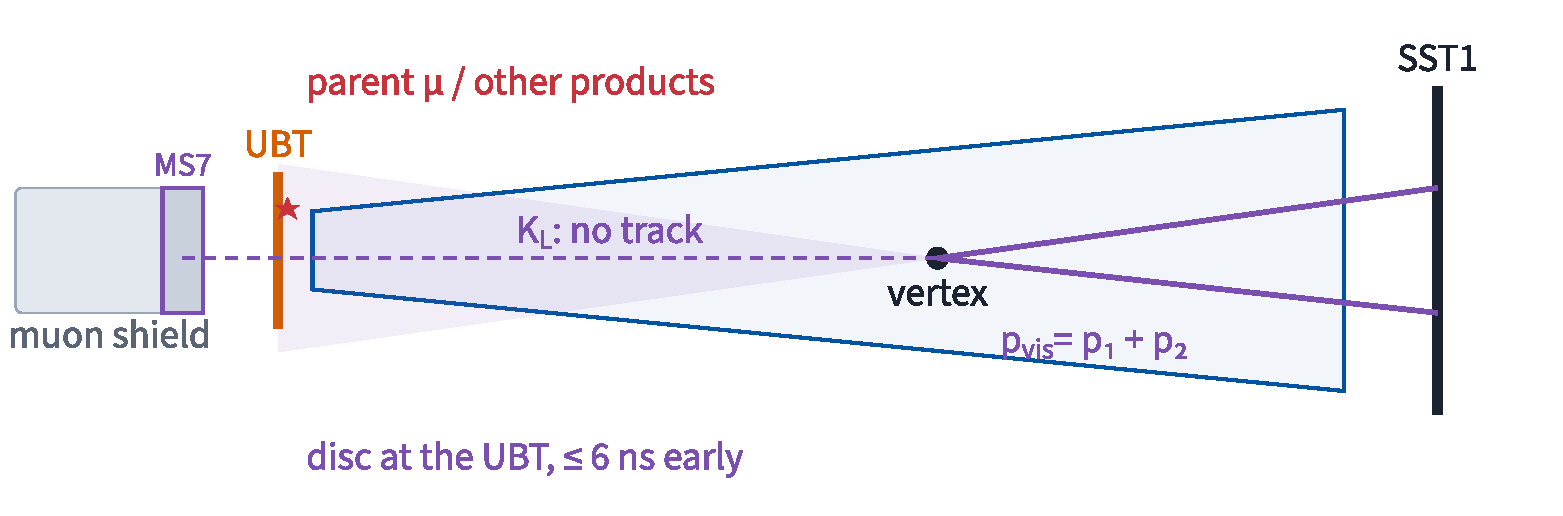
\includegraphics[width=1.00\linewidth,height=59.18pt,keepaspectratio]{figs/s22_sk1.pdf}\par}
\end{minipage}%
\hfill%
\begin{minipage}[c]{\dimexpr(0.4000\linewidth-0.4000\dimexpr7.85pt\relax)}\raggedright
\begin{mathbox}[purple]{5.23pt}
\textbf{neutral back-trace}\newline{}r = 5 cm + max(25 mrad, 0.25 GeV / p\textsubscript{vis}) · Δz\newline{}−w − t\textsubscript{early} < Δt < w, t\textsubscript{early} ≤ 6 ns\newline{}\textcolor{muted}{Δz: from the vertex back to the plane}
\end{mathbox}
\end{minipage}\par
\vspace{2.46pt}
{\fontsize{4.55pt}{6.37pt}\selectfont
\begin{itemize}
  \item A K\textsubscript{L} made upstream leaves no track: only its decay pair is seen
  \item Trace back from the vertex along p\textsubscript{vis}: vertex at 50 m → UBT, Δz ≈ 19 m\newline{}p\textsubscript{vis} = 15 GeV: θ = 25 mrad, r = 5 cm + 25 mrad × 19 m ≈ \textbf{0.5 m}\newline{}p\textsubscript{vis} = 5 GeV: θ = 50 mrad, r ≈ \textbf{1.0 m}
  \item The K\textsubscript{L} is slow: the window opens up to its flight time earlier (≤ 6 ns). Any hit (parent muon, sister particles) → \textbf{tagged}
\end{itemize}}
\end{btframe}

% ---------------------------------------------------------------- slide 24: How a candidate is tagged: MS7 strips
\begin{btframe}{5 · Background tagging · tagging chain 3/3}{How a candidate is tagged: MS7 strips}
\fadeblock{0.28}{\noindent \begin{minipage}[c]{38.69pt}\raggedright
{\fontsize{4.32pt}{5.84pt}\selectfont \textcolor{cern}{\textbf{Tracks}}\par}
\end{minipage}%
\hfill%
\begin{minipage}[c]{\dimexpr(1.0000\linewidth-1.0000\dimexpr42.90pt\relax)}\raggedright
\begin{flowrow}{\dimexpr(\linewidth-3\dimexpr5.46pt\relax)/4\relax}{5.46pt}%
\flowstep{white}{rule}{2.28pt}{3.64pt}{{\fontsize{4.78pt}{5.97pt}\selectfont\textbf{\textcolor{cern}{candidate}}\par}\vspace{0.91pt}{\fontsize{4.10pt}{5.53pt}\selectfont\textcolor{ink}{2 tracks, vertex in the vessel}\par}}%
\flowarrow%
\flowstep{white}{rule}{2.28pt}{3.64pt}{{\fontsize{4.78pt}{5.97pt}\selectfont\textbf{\textcolor{cern}{each track back}}\par}\vspace{0.91pt}{\fontsize{4.10pt}{5.53pt}\selectfont\textcolor{ink}{straight line from SST1 upstream}\par}}%
\flowarrow%
\flowstep{white}{rule}{2.28pt}{3.64pt}{{\fontsize{4.78pt}{5.97pt}\selectfont\textbf{\textcolor{cern}{window}}\par}\vspace{0.91pt}{\fontsize{4.10pt}{5.53pt}\selectfont\textcolor{ink}{r = 5 cm + (0.5 + 6 GeV/p) mrad·Δz, ±3σ}\par}}%
\flowarrow%
\flowstep{white}{rule}{2.28pt}{3.64pt}{{\fontsize{4.78pt}{5.97pt}\selectfont\textbf{\textcolor{cern}{hit?}}\par}\vspace{0.91pt}{\fontsize{4.10pt}{5.53pt}\selectfont\textcolor{ink}{yes → tagged}\par}}%
\end{flowrow}
\end{minipage}\par
}\vspace{2.46pt}
\fadeblock{0.28}{\noindent \begin{minipage}[c]{38.69pt}\raggedright
{\fontsize{4.32pt}{5.84pt}\selectfont \textcolor{purple}{\textbf{Neutrals (V0 rule, R2, R3)}}\par}
\end{minipage}%
\hfill%
\begin{minipage}[c]{\dimexpr(1.0000\linewidth-1.0000\dimexpr42.90pt\relax)}\raggedright
\begin{flowrow}{\dimexpr(\linewidth-3\dimexpr5.46pt\relax)/4\relax}{5.46pt}%
\flowstep{white}{rule}{2.28pt}{3.64pt}{{\fontsize{4.78pt}{5.97pt}\selectfont\textbf{\textcolor{purple}{candidate}}\par}\vspace{0.91pt}{\fontsize{4.10pt}{5.53pt}\selectfont\textcolor{ink}{p\textsubscript{vis} < 20 GeV}\par}}%
\flowarrow%
\flowstep{white}{rule}{2.28pt}{3.64pt}{{\fontsize{4.78pt}{5.97pt}\selectfont\textbf{\textcolor{purple}{trace back as a neutral}}\par}\vspace{0.91pt}{\fontsize{4.10pt}{5.53pt}\selectfont\textcolor{ink}{vertex → UBT along p\textsubscript{vis}}\par}}%
\flowarrow%
\flowstep{white}{rule}{2.28pt}{3.64pt}{{\fontsize{4.78pt}{5.97pt}\selectfont\textbf{\textcolor{purple}{disc + early window}}\par}\vspace{0.91pt}{\fontsize{4.10pt}{5.53pt}\selectfont\textcolor{ink}{5 cm + max(25, 250/p\textsubscript{vis}) mrad·Δz}\par}}%
\flowarrow%
\flowstep{white}{rule}{2.28pt}{3.64pt}{{\fontsize{4.78pt}{5.97pt}\selectfont\textbf{\textcolor{purple}{any hit?}}\par}\vspace{0.91pt}{\fontsize{4.10pt}{5.53pt}\selectfont\textcolor{ink}{yes → tagged}\par}}%
\end{flowrow}
\end{minipage}\par
}\vspace{2.46pt}
\noindent \begin{minipage}[c]{38.69pt}\raggedright
{\fontsize{4.32pt}{5.84pt}\selectfont \textcolor{red}{\textbf{MS7 (MSMS, R3)}}\par}
\end{minipage}%
\hfill%
\begin{minipage}[c]{\dimexpr(1.0000\linewidth-1.0000\dimexpr42.90pt\relax)}\raggedright
\begin{flowrow}{\dimexpr(\linewidth-3\dimexpr5.46pt\relax)/4\relax}{5.46pt}%
\flowstep{red}{red}{2.28pt}{3.64pt}{{\fontsize{4.78pt}{5.97pt}\selectfont\textbf{\textcolor{white}{candidate}}\par}\vspace{0.91pt}{\fontsize{4.10pt}{5.53pt}\selectfont\textcolor{white}{traced back as a neutral}\par}}%
\flowarrow%
\flowstep{red}{red}{2.28pt}{3.64pt}{{\fontsize{4.78pt}{5.97pt}\selectfont\textbf{\textcolor{white}{strip layers}}\par}\vspace{0.91pt}{\fontsize{4.10pt}{5.53pt}\selectfont\textcolor{white}{29.39 / 29.59 / 29.79 m}\par}}%
\flowarrow%
\flowstep{red}{red}{2.28pt}{3.64pt}{{\fontsize{4.78pt}{5.97pt}\selectfont\textbf{\textcolor{white}{disc}}\par}\vspace{0.91pt}{\fontsize{4.10pt}{5.53pt}\selectfont\textcolor{white}{2 cm + 10 mrad·Δz, ±1.5 ns}\par}}%
\flowarrow%
\flowstep{red}{red}{2.28pt}{3.64pt}{{\fontsize{4.78pt}{5.97pt}\selectfont\textbf{\textcolor{white}{own products?}}\par}\vspace{0.91pt}{\fontsize{4.10pt}{5.53pt}\selectfont\textcolor{white}{yes → tagged}\par}}%
\end{flowrow}
\end{minipage}\par
\vspace{2.46pt}
\noindent \begin{minipage}[c]{\dimexpr(0.6000\linewidth-0.6000\dimexpr7.85pt\relax)}\raggedright
{\centering 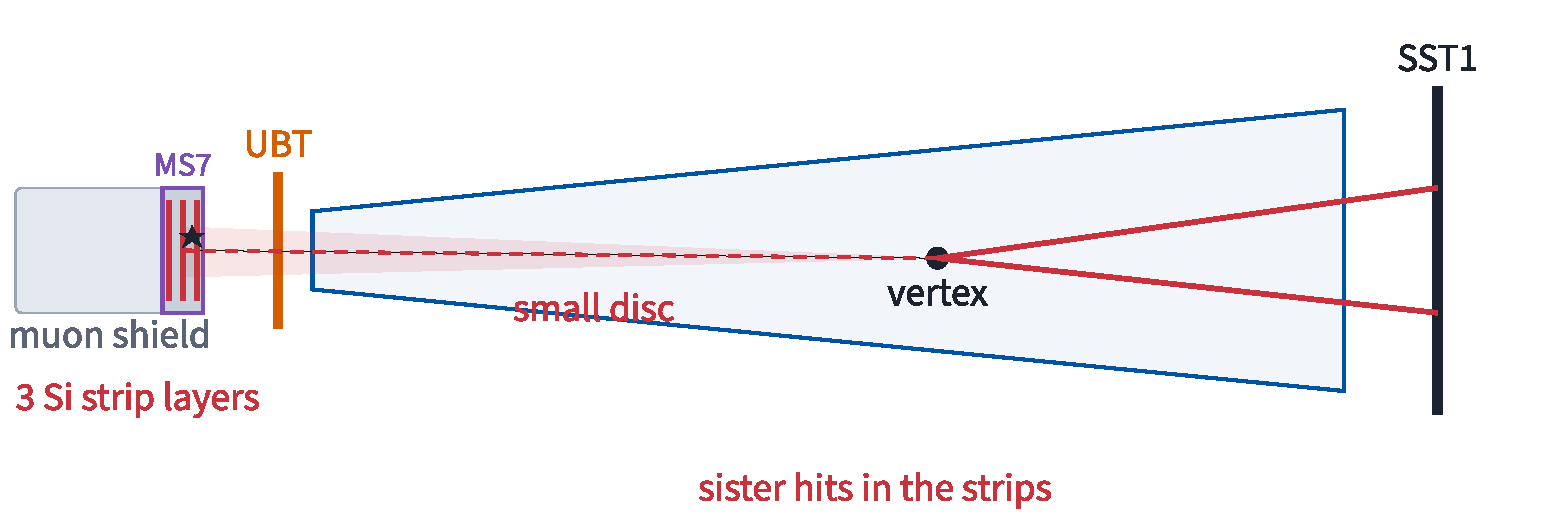
\includegraphics[width=1.00\linewidth,height=59.18pt,keepaspectratio]{figs/s23_sk1.pdf}\par}
\end{minipage}%
\hfill%
\begin{minipage}[c]{\dimexpr(0.4000\linewidth-0.4000\dimexpr7.85pt\relax)}\raggedright
\begin{mathbox}[red]{5.23pt}
\textbf{strip disc}\newline{}r = 2 cm + 10 mrad · Δz\newline{}|Δt| < 1.5 ns\newline{}\textcolor{muted}{Δz: from the vertex back to the strip layer}
\end{mathbox}
\end{minipage}\par
\vspace{2.46pt}
{\fontsize{4.55pt}{6.37pt}\selectfont
\begin{itemize}
  \item K\textsubscript{L} made in the last iron (MS7) by the muon: the parent muon and other products cross the strips
  \item Same back-trace, but the strips are close and precise: vertex at 50 m → MS7 (29.6 m), Δz ≈ 20 m\newline{}r = 2 cm + 10 mrad × 20 m ≈ \textbf{22 cm}, ±1.5 ns
  \item Own products in the disc → \textbf{tagged}. At full selection the V0 rule alone already leaves 0.67 ± 0.32 MS7 events (R2 = R3); the strips help the partial selection: 4.7×10\textsuperscript{4} → 3.6×10\textsuperscript{4}
  \item Applied to \textbf{every} candidate: the origin is not assumed. A candidate not made in MS7 has no strip hits on its line, except by chance (that is the random-hit cost)
\end{itemize}}
\end{btframe}

% ---------------------------------------------------------------- slide 25: Slow MS7 KL escaped the 25 mrad cone: three fixes, A + C adopted
\begin{btframe}{5 · Background tagging · V0 rule fixes}{Slow MS7 K\textsubscript{L} escaped the 25 mrad cone: three fixes, A + C adopted}
\noindent \begin{minipage}[t]{\dimexpr(0.2500\linewidth-0.2500\dimexpr14.22pt\relax)}\vspace{0pt}\raggedright
{\centering \fontsize{4.55pt}{6.15pt}\selectfont \textcolor{purple}{\textbf{25 mrad cone: misses (slow K\textsubscript{L})}}\par}
\vspace{0.27pt}
{\centering 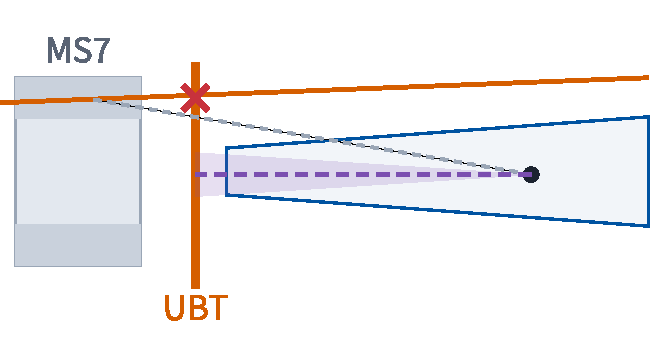
\includegraphics[width=1.00\linewidth,height=63.73pt,keepaspectratio]{figs/s24_sk1.pdf}\par}
\end{minipage}%
\hfill%
\begin{minipage}[t]{\dimexpr(0.2500\linewidth-0.2500\dimexpr14.22pt\relax)}\vspace{0pt}\raggedright
{\centering \fontsize{4.55pt}{6.15pt}\selectfont \textcolor{purple}{\textbf{A: cone max(25 mrad, 0.25 GeV / p\textsubscript{vis})}}\par}
\vspace{0.27pt}
{\centering 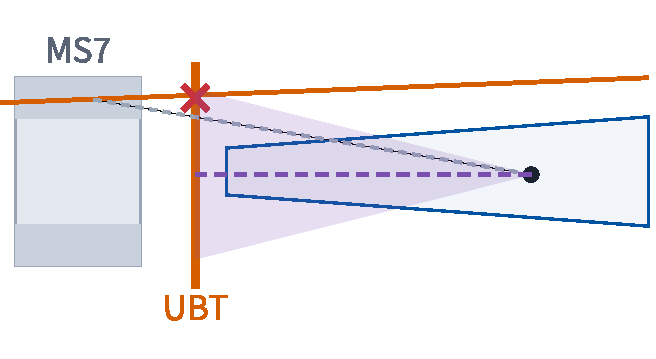
\includegraphics[width=1.00\linewidth,height=63.73pt,keepaspectratio]{figs/s24_sk2.pdf}\par}
\end{minipage}%
\hfill%
\begin{minipage}[t]{\dimexpr(0.2500\linewidth-0.2500\dimexpr14.22pt\relax)}\vspace{0pt}\raggedright
{\centering \fontsize{4.55pt}{6.15pt}\selectfont \textcolor{purple}{\textbf{B: extra lines to the yoke legs}}\par}
\vspace{0.27pt}
{\centering 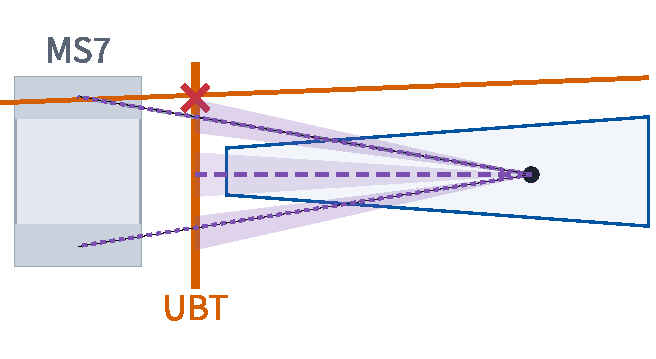
\includegraphics[width=1.00\linewidth,height=63.73pt,keepaspectratio]{figs/s24_sk3.pdf}\par}
\end{minipage}%
\hfill%
\begin{minipage}[t]{\dimexpr(0.2500\linewidth-0.2500\dimexpr14.22pt\relax)}\vspace{0pt}\raggedright
{\centering \fontsize{4.55pt}{6.15pt}\selectfont \textcolor{purple}{\textbf{C: window opened by the K\textsubscript{L} flight time}}\par}
\vspace{0.27pt}
{\centering 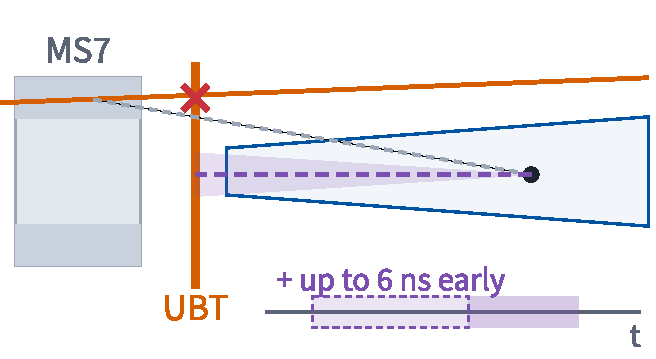
\includegraphics[width=1.00\linewidth,height=63.73pt,keepaspectratio]{figs/s24_sk4.pdf}\par}
\end{minipage}\par
\vspace{2.46pt}
{\fontsize{4.37pt}{5.68pt}\selectfont\setlength{\tabcolsep}{3.06pt}\renewcommand{\arraystretch}{1.42}
\begin{tabularx}{\linewidth}{>{\raggedright\arraybackslash}Xrrrr}
\textcolor{muted}{variant} & \textcolor{muted}{signal lost F / P} & \textcolor{muted}{MS7 μ tagged} & \textcolor{muted}{own hits only} & \textcolor{muted}{MS7 μ left / 15 y} \\\headrule
R3 with 25 mrad & 5.3 / 9.4 \% & 66 \% & 63 \% & 8.1×10\textsuperscript{3} \\\rowrule
A: 1/p cone & 5.4 / 10.5 \% & 100 \% & 100 \% & 0.63 \\\rowrule
B: yoke lines & 12.1 / 25.1 \% & 100 \% & 100 \% & 0.48 \\\rowrule
C: time of flight & 4.9 / 7.6 \% & 68 \% & 67 \% & 7.8×10\textsuperscript{3} \\\rowrule
\rowcolor{tint}\bfseries A + C (adopted, R3) & \bfseries 5.0 / 8.4 \% & \bfseries 100 \% & \bfseries 100 \% & \bfseries 0.67 \\\rowrule
B + C & 11.5 / 21.8 \% & 100 \% & 100 \% & 0.48 \\\rowrule
\end{tabularx}\par}
\slidenote{Source: results\_rerun/r3\_escapes/variants/v0study\_variants.json and v0study\_variants\_ownhits.json (bin/v0rule\_study.py, code 2e228bf); signal: results\_rerun/reco/r3var\_*.json (bin/run\_reco.py). Before the D19 energy loss and SBT ×4.}
\end{btframe}

% ---------------------------------------------------------------- slide 26: The SBT model: material, rules, energy loss, random rate
\begin{btframe}{5 · Background tagging · SBT model}{The SBT model: material, rules, energy loss, random rate}
{\fontsize{4.74pt}{6.16pt}\selectfont\setlength{\tabcolsep}{3.32pt}\renewcommand{\arraystretch}{1.42}
\begin{tabularx}{\linewidth}{l>{\raggedright\arraybackslash}Xr}
\textcolor{muted}{ingredient} & \textcolor{muted}{what} & \textcolor{muted}{effect (R2)} \\\headrule
SBT material as a target (Al / LS / ribs) & 1.2×10\textsuperscript{4} μ-induced candidates / 15 y (IP < 10 cm) & new background class \\\rowrule
v0\_line + self-tag & own LS deposits of the interaction & 783 → 113 (SBT rules alone) \\\rowrule
zone rule & in-time cell downstream of the vertex & ν in helium 3.5 → 1.1; signal −0.6 \% (×1) / −2.3 \% (×4) \\\rowrule
scattering in the shell (k = 1) & kick at the exit of each shell piece & single μ tagging 92 → 85 \% \\\rowrule
mean energy loss in the shell & Al 0.436, LS 0.150 GeV/m; soft muons stop & 45 \% of single-μ weight stops; tagging → 95 \%; pairs 2.36 → 1.14 \\\rowrule
random rate ×4 & cavern back-scatter, e / γ (SR-389: ×13) & signal +2 points (zone rule) \\\rowrule
\end{tabularx}\par}
\slidenote{Source: veto docs/d19\_sbt.md sections 4–8, ISSUES D19 (closed 17 Nov); results\_rerun/sbt\_d19/flags17/ and sbt\_d19/rangeout/summary\_R2.json (bin/sbt\_eval.py, bin/run\_reco.py; Slurm 2112324).}
\end{btframe}

% ---------------------------------------------------------------- slide 27: R1: UBT only — 99.7 drachmas, 18 100 channels
\begin{btframe}{5 · Background tagging · R1}{R1: UBT only — 99.7 drachmas, 18 100 channels}
{\centering \designsketch[54.62pt]{}{0}{}\par}
\vspace{2.46pt}
\noindent \begin{minipage}[t]{\dimexpr(0.5556\linewidth-0.5556\dimexpr11.49pt\relax)}\vspace{0pt}\raggedright
{\fontsize{5.31pt}{6.90pt}\selectfont\setlength{\tabcolsep}{3.72pt}\renewcommand{\arraystretch}{1.42}
\begin{tabular}{lr}
\textcolor{muted}{per 15 y, full selection} & \textcolor{muted}{R1} \\\headrule
signal lost, full / partial IP cut & 2.45 / 2.24 \% (4.0 / 3.8 at UBT rate ×2) \\\rowrule
μμ pairs & < 0.26 (90 \% CL) \\\rowrule
rock × μ pairs & 0.59 ± 0.09 \\\rowrule
interaction product × μ pairs & 0.019 ± 0.002 \\\rowrule
μ in the vessel & 70 ± 8 \\\rowrule
ν in the vessel & 3.5 \\\rowrule
MS7 μ (V0, K\textsuperscript{±}) & 1.70×10\textsuperscript{4} \\\rowrule
ν in MS7 & 2.6 \\\rowrule
\end{tabular}\par}
\end{minipage}%
\hfill%
\begin{minipage}[t]{\dimexpr(0.4444\linewidth-0.4444\dimexpr11.49pt\relax)}\vspace{0pt}\raggedright
{\fontsize{6.15pt}{8.60pt}\selectfont
\begin{itemize}
  \item Straws on the window + 4 × 4 m\textsuperscript{2} tile plane (2 × 2 cm\textsuperscript{2} in the flames)
  \item Catches what enters through the entrance window; blind to the side walls (rock tracks, bounced muons)
  \item Signal loss: 1.5 points EM debris on the straws, 1 point muons in the flame tiles
\end{itemize}}
\end{minipage}\par
\slidenote{Source: results\_rerun/reco/reco\_R1\_ubt\_only\_\{full,partial\}\_base0eb5209[\_ubtx2].json (bin/run\_reco.py), r123\_ms7\_base0eb5209.json (bin/v0rule\_study.py, MS7), r123\_vessel\_d19\_d3065c3.json (vessel μ/ν, bin/vessel\_prepare.py caches), sbt\_d19/rangeout/summary\_*.json, rock\_comb\_*\_ul90\_0030e68.json; code 0eb5209.}
\end{btframe}

% ---------------------------------------------------------------- slide 28: R2: SBT + UBT + V0 rule — 333.5 drachmas (the budget), 31 764 channels
\begin{btframe}{5 · Background tagging · R2}{R2: SBT + UBT + V0 rule — 333.5 drachmas (the budget), 31 764 channels}
{\centering \designsketch[54.62pt]{0,...,9}{0}{SBT: 10 rings, 854 liquid-scintillator cells on the four walls}\par}
\vspace{2.46pt}
\noindent \begin{minipage}[t]{\dimexpr(0.5556\linewidth-0.5556\dimexpr11.49pt\relax)}\vspace{0pt}\raggedright
{\fontsize{5.31pt}{6.90pt}\selectfont\setlength{\tabcolsep}{3.72pt}\renewcommand{\arraystretch}{1.42}
\begin{tabular}{lr}
\textcolor{muted}{per 15 y, full selection} & \textcolor{muted}{R2} \\\headrule
signal lost, full / partial IP cut & 6.7 / 9.7 \% (9.3 / 14.1 at UBT rate ×2) \\\rowrule
μμ pairs & < 0.052 (90 \% CL) \\\rowrule
rock × μ pairs & < 0.018 (90 \% CL) \\\rowrule
interaction product × μ pairs & < 1.1×10\textsuperscript{-4} \\\rowrule
μ in the vessel & 1.3 ± 1.3 (1 event) \\\rowrule
ν in the vessel & 1.09 ± 0.10 \\\rowrule
SBT material μ / ν & 0 (K\textsubscript{L} < 13) / 0.05 \\\rowrule
\rowcolor{tint}\bfseries MS7 μ (V0, K\textsuperscript{±}) & \bfseries 0.67 ± 0.32 \\\rowrule
ν in MS7 & 0.70 \\\rowrule
\end{tabular}\par}
\end{minipage}%
\hfill%
\begin{minipage}[t]{\dimexpr(0.4444\linewidth-0.4444\dimexpr11.49pt\relax)}\vspace{0pt}\raggedright
{\fontsize{6.15pt}{8.60pt}\selectfont
\begin{itemize}
  \item Removes everything entering through the walls: pairs, rock, vessel μ
  \item Single SST1 muons tagged 95 \%
  \item \textbf{V0 rule} (A+C, software only): MS7 1.8×10\textsuperscript{4} → \textbf{0.67}, SBT-material K\textsubscript{L} 112 → < 13
  \item Cost of the V0 rule: signal 5.0 / 5.2 → 6.7 / 9.7 \%
\end{itemize}}
\end{minipage}\par
\slidenote{Source: R2 with the V0 rule (designs/R2\_sbt\_ubt.json detector.v0\_rule, 18 Nov 2026; Slurm 2125101): results\_rerun/reco/reco\_R2\_sbt\_ubt\_\{full,partial\}\_r2v0[\_ubtx2].json (bin/run\_reco.py), r2v0\_ms7.json, r2v0\_vessel\_d19.json (bin/v0rule\_study.py), sbt\_d19/rangeout\_r2v0/summary\_R2.json (bin/sbt\_eval.py, bin/sbt\_summary.py), rock\_comb\_R2\_sbt\_ubt\_r2v0.json.}
\end{btframe}

% ---------------------------------------------------------------- slide 29: R3: R2 + Muon Shield Monitoring System — 378.7 drachmas
\begin{btframe}{5 · Background tagging · R3}{R3: R2 + Muon Shield Monitoring System — 378.7 drachmas}
{\centering \designsketch[45.52pt]{0,...,9}{1}{SBT: 10 rings, 854 liquid-scintillator cells on the four walls}\par}
\vspace{2.46pt}
\noindent \begin{minipage}[t]{\dimexpr(0.5405\linewidth-0.5405\dimexpr11.49pt\relax)}\vspace{0pt}\raggedright
{\fontsize{5.31pt}{6.90pt}\selectfont\setlength{\tabcolsep}{3.72pt}\renewcommand{\arraystretch}{1.42}
\begin{tabular}{lr}
\textcolor{muted}{per 15 y, full selection} & \textcolor{muted}{R3} \\\headrule
signal lost, full / partial IP cut & 6.8 / 10.2 \% (9.2 / 14.9 at UBT rate ×2) \\\rowrule
μμ, rock × μ pairs & < 0.052, < 0.018 \\\rowrule
interaction product × μ pairs & < 1.1×10\textsuperscript{-4} (≤ R2) \\\rowrule
μ in the vessel & 1.3 ± 1.3 (1 event) \\\rowrule
ν in the vessel & 1.09 ± 0.10 \\\rowrule
SBT material μ / ν & 0 (K\textsubscript{L} < 13) / 0.05 \\\rowrule
\rowcolor{tint}\bfseries MS7 μ (V0, K\textsuperscript{±}) & \bfseries 0.7 ± 0.3 \\\rowrule
ν in MS7 & 0.70 \\\rowrule
\end{tabular}\par}
\end{minipage}%
\hfill%
\begin{minipage}[t]{\dimexpr(0.4595\linewidth-0.4595\dimexpr11.49pt\relax)}\vspace{0pt}\raggedright
{\fontsize{6.15pt}{8.60pt}\selectfont
\begin{itemize}
  \item \textbf{Why MSMS:} the MS7 K\textsubscript{L} are the largest background and neutral; the only handle is the interaction itself, inside the last iron: 3 × 8 strip stations (30 × 30 cm\textsuperscript{2}) on the return-yoke legs, 82 \% of the V0 interaction points
  \item On top of R2 (with the V0 rule) the strips change nothing at full selection; partial selection MS7 4.7×10\textsuperscript{4} → 3.6×10\textsuperscript{4}
  \item +45 drachmas over the budget
\end{itemize}}
\end{minipage}\par
\slidenote{Source: results\_rerun/reco/reco\_R3\_sbt\_ubt\_strips\_\{full,partial\}\_base0eb5209[\_ubtx2].json (bin/run\_reco.py), r123\_ms7\_base0eb5209.json (bin/v0rule\_study.py, MS7), r123\_vessel\_d19\_d3065c3.json (vessel μ/ν, bin/vessel\_prepare.py caches), sbt\_d19/rangeout/summary\_*.json, rock\_comb\_*\_ul90\_0030e68.json; code 0eb5209.}
\end{btframe}

% ---------------------------------------------------------------- slide 30: R1, R2, R3: background left in 15 years and signal lost
\begin{btframe}{5 · Background tagging · summary}{R1, R2, R3: background left in 15 years and signal lost}
{\fontsize{5.31pt}{6.90pt}\selectfont\setlength{\tabcolsep}{3.72pt}\renewcommand{\arraystretch}{1.42}
\begin{tabularx}{\linewidth}{>{\raggedright\arraybackslash}Xrrr}
\textcolor{muted}{per 15 y, full selection} & \textcolor{muted}{R1} & \textcolor{muted}{R2} & \textcolor{muted}{R3} \\\headrule
μμ pairs & < 0.26 & < 0.052 & < 0.052 \\\rowrule
rock × μ pairs & 0.59 & < 0.018 & < 0.018 \\\rowrule
interaction product × μ pairs & 0.019 & < 1.1×10\textsuperscript{-4} & < 1.1×10\textsuperscript{-4} \\\rowrule
μ in the vessel (helium, walls) & 70 & 1.3 (1 ev.) & 1.3 (1 ev.) \\\rowrule
SBT material, K\textsubscript{L} / other & – & < 13 / < 940 & < 13 / < 940 \\\rowrule
MS7 μ (V0, K\textsuperscript{±}) & 1.70×10\textsuperscript{4} & 0.67 ± 0.32 & 0.7 ± 0.3 \\\rowrule
ν in the vessel & 3.5 & 1.09 & 1.09 \\\rowrule
ν in MS7 / SBT material & 2.6 / – & 0.70 / 0.05 & 0.70 / 0.05 \\\rowrule
\rowcolor{tint}\bfseries signal lost, full / partial IP cut & \bfseries 2.45 / 2.24 \% & \bfseries 6.74 / 9.71 \% & \bfseries 6.83 / 10.16 \% \\\rowrule
\rowcolor{tint}\bfseries signal lost at UBT rate ×2 & \bfseries 3.98 / 3.83 \% & \bfseries 9.33 / 14.14 \% & \bfseries 9.17 / 14.88 \% \\\rowrule
\end{tabularx}\par}
\vspace{2.46pt}
{\fontsize{6.15pt}{8.60pt}\selectfont
\begin{itemize}
  \item “<”: no simulated event left, 90 \% CL upper limit 2.30 Σw\textsuperscript{2}/Σw
  \item With the V0 rule, R2 leaves the same background as R3: the MSMS strips only help the partial selection
  \item Signal is lost only to random hits in the search windows: the V0 disc is the most sensitive (+2.6 / +4.4 points at twice the UBT rate)
\end{itemize}}
\slidenote{Source: R1, R3 report Table 7 (tab:tag:eff), code 0eb5209; R2 with the V0 rule: the *\_r2v0 files (Slurm 2125101); signal at UBT ×2: reco\_R*\_\{full,partial\}\_base0eb5209\_ubtx2.json (bin/run\_reco.py --plane-rate-scale 2). Interactions in the tagger planes themselves (350 μ, 3.4 ν before tagging) not yet included.}
\end{btframe}

% ---------------------------------------------------------------- slide 31: Z2: R2 without the SBT, 7 straw fins per side — 439.7 drachmas, 193 368 channels
\begin{btframe}{5 · Background tagging · Z2}{Z2 (optimised): SBT 6 rings + UBT + V0 rule — 225.3 drachmas, 21 171 channels}
{\centering {\renewcommand{\skubtlabel}{UBT: straws + tiles |x| < 1.7 m, 2 × 2 cm\textsuperscript{2} only on the cavern side}\designsketch[45.52pt]{2,5,6,7,8,9}{0}{SBT: rings 2, 5–9 (6 of 10)}}\par}
\vspace{2.46pt}
\noindent \begin{minipage}[t]{\dimexpr(0.5556\linewidth-0.5556\dimexpr11.49pt\relax)}\vspace{0pt}\raggedright
{\fontsize{5.31pt}{6.90pt}\selectfont\setlength{\tabcolsep}{3.72pt}\renewcommand{\arraystretch}{1.42}
\begin{tabular}{lr}
\textcolor{muted}{per 15 y, full selection} & \textcolor{muted}{Z2} \\\headrule
signal lost, full IP cut & 2.71 \% \\\rowrule
combinatorial pairs & 0 simulated pairs left \\\rowrule
μ in the vessel & 1.3 ± 1.3 (1 event) \\\rowrule
ν in the helium & 1.13 ± 0.11 \\\rowrule
SBT material & 0.004 ± 0.003 \\\rowrule
\rowcolor{tint}\bfseries MS7 (μ V0, K\textsuperscript{±}, ν) & \bfseries 0.80 ± 0.34 \\\rowrule
single SST1 muons tagged, all / bounced & 91 / 84 \% \\\rowrule
\end{tabular}\par}
\end{minipage}%
\hfill%
\begin{minipage}[t]{\dimexpr(0.4444\linewidth-0.4444\dimexpr11.49pt\relax)}\vspace{0pt}\raggedright
{\fontsize{6.15pt}{8.60pt}\selectfont
\begin{itemize}
  \item Best design of the genetic-algorithm search (section 6): R2 with 6 of the 10 SBT rings (no 0, 1, 3, 4)
  \item UBT straws with t\textsubscript{0} and the segment cut; tile plane |x| < 1.7 m, 2×2 cm only on the cavern side
  \item V0 rule with a 15.7 mrad cone, no K\textsubscript{L} time-of-flight window, p\textsubscript{max} kept
  \item \textbf{Signal loss 2.7 \%} (R2: 6.7 \%), 68 \% of the budget; every plane within its rate limit
\end{itemize}}
\end{minipage}\par
\slidenote{Optimised design (ga7c3 of run results\_rerun/evolve/ga\_20261119\_115533, re-scored −71.0 ± 0.5 over 3 seeds); design file results\_rerun/evolve/Z2\_opt\_ga7c3.json. Evaluated with the optimiser chain (full selection, UBT rate ×1). The vessel μ is the single helium event of R2; the SBT-material gain over the seed is one heavy event.}
\end{btframe}

% ---------------------------------------------------------------- slide 32: Z3 (optimised)
\begin{btframe}{5 · Background tagging · Z3}{Z3 (optimised): SBT 7 rings + UBT + V0 rule — 244.7 drachmas, 22 428 channels}
{\centering {\renewcommand{\skubtlabel}{UBT: straws + tiles |x| < 1.7 m, 2 × 2 cm\textsuperscript{2} only on the cavern side}\designsketch[45.52pt]{2,3,5,6,7,8,9}{0}{SBT: rings 2, 3, 5–9 (7 of 10)}}\par}
\vspace{2.46pt}
\noindent \begin{minipage}[t]{\dimexpr(0.5556\linewidth-0.5556\dimexpr11.49pt\relax)}\vspace{0pt}\raggedright
{\fontsize{5.31pt}{6.90pt}\selectfont\setlength{\tabcolsep}{3.72pt}\renewcommand{\arraystretch}{1.42}
\begin{tabular}{lr}
\textcolor{muted}{per 15 y, full selection} & \textcolor{muted}{Z3} \\\headrule
signal lost, full IP cut & 3.01 \% \\\rowrule
combinatorial pairs & 0 simulated pairs left \\\rowrule
μ in the vessel & 1.3 ± 1.3 (1 event) \\\rowrule
ν in the helium & 1.05 ± 0.10 \\\rowrule
SBT material & 0.004 ± 0.003 \\\rowrule
\rowcolor{tint}\bfseries MS7 (μ V0, K\textsuperscript{±}, ν) & \bfseries 0.61 ± 0.27 \\\rowrule
single SST1 muons tagged, all / bounced & 94 / 84 \% \\\rowrule
\end{tabular}\par}
\end{minipage}%
\hfill%
\begin{minipage}[t]{\dimexpr(0.4444\linewidth-0.4444\dimexpr11.49pt\relax)}\vspace{0pt}\raggedright
{\fontsize{6.15pt}{8.60pt}\selectfont
\begin{itemize}
  \item Second design of the search: as Z2 with ring 3 back (7 rings)
  \item MS7 0.61 and single SST1 tagging 94 \% (Z2: 0.80, 91 \%) for +19 drachmas
  \item \textbf{Signal loss 3.0 \%}, 73 \% of the budget
\end{itemize}}
\end{minipage}\par
\slidenote{Optimised design (ga8c8 of run results\_rerun/evolve/ga\_20261119\_115533, re-scored −75.9 ± 5.9 over 3 seeds); design file results\_rerun/evolve/Z3\_opt\_ga8c8.json. Evaluated with the optimiser chain (full selection, UBT rate ×1).}
\end{btframe}

% ---------------------------------------------------------------- slide 33: What R2 and R3 leave, and what is not yet known
\begin{btframe}{5 · Background tagging · what is left}{What R2 and R3 leave, and what is not yet known}
{\fontsize{6.15pt}{8.60pt}\selectfont
\begin{itemize}
  \item \textbf{Neutrinos in the helium} (1.1 / 15 y): no charged particle upstream; the zone rule removes two thirds
  \item \textbf{Neutrinos in MS7} (0.7 / 15 y)
  \item \textbf{Statistics}: μμ pairs < 0.05, vessel walls < 49, SBT non-K\textsubscript{L} < 940 per 15 y at 90 \% CL: not yet shown to be below 0.1; enriched samples needed
\end{itemize}}
\slidenote{Source: results\_rerun/closure/mu\_he\_survivor.json (bin/mu\_he\_survivor\_diag.py on prepared\_muon\_nov4full\_d19); 90 \% CL limits from the sample weights (veto interactions.ul90, code 0030e68).}
\end{btframe}
